\documentclass[xcolor={dvipsnames}]{beamer}
\usepackage[utf8]{inputenc}
\usepackage{amsmath, amssymb, upgreek}
\usepackage{graphicx, float, subcaption}
\usepackage{hyperref}

\graphicspath{{Figures/}}

\usetheme{default}


\title{Introduction to Scientific Computing}


\author{Pablo Brubeck\inst{}}
\institute[ITESM]
{
  \inst{}
  Department of Physics\\
  Tecnologico de Monterrey
}

\date{\today}
\subject{Numerical Analysis}

\AtBeginSection[]
{
  \begin{frame}<beamer>{Outline}
    \tableofcontents[currentsection]
  \end{frame}
}

\begin{document}

\begin{frame}
  \titlepage
\end{frame}

\begin{frame}{Outline}
  \tableofcontents
  % You might wish to add the option [pausesections]
\end{frame}


\section{The Big Picture}

\begin{frame}{Ada Lovelace wrote the first computer program in 1842\\ to calculate the Bernoulli Numbers.}{}
\begin{figure}
\centering
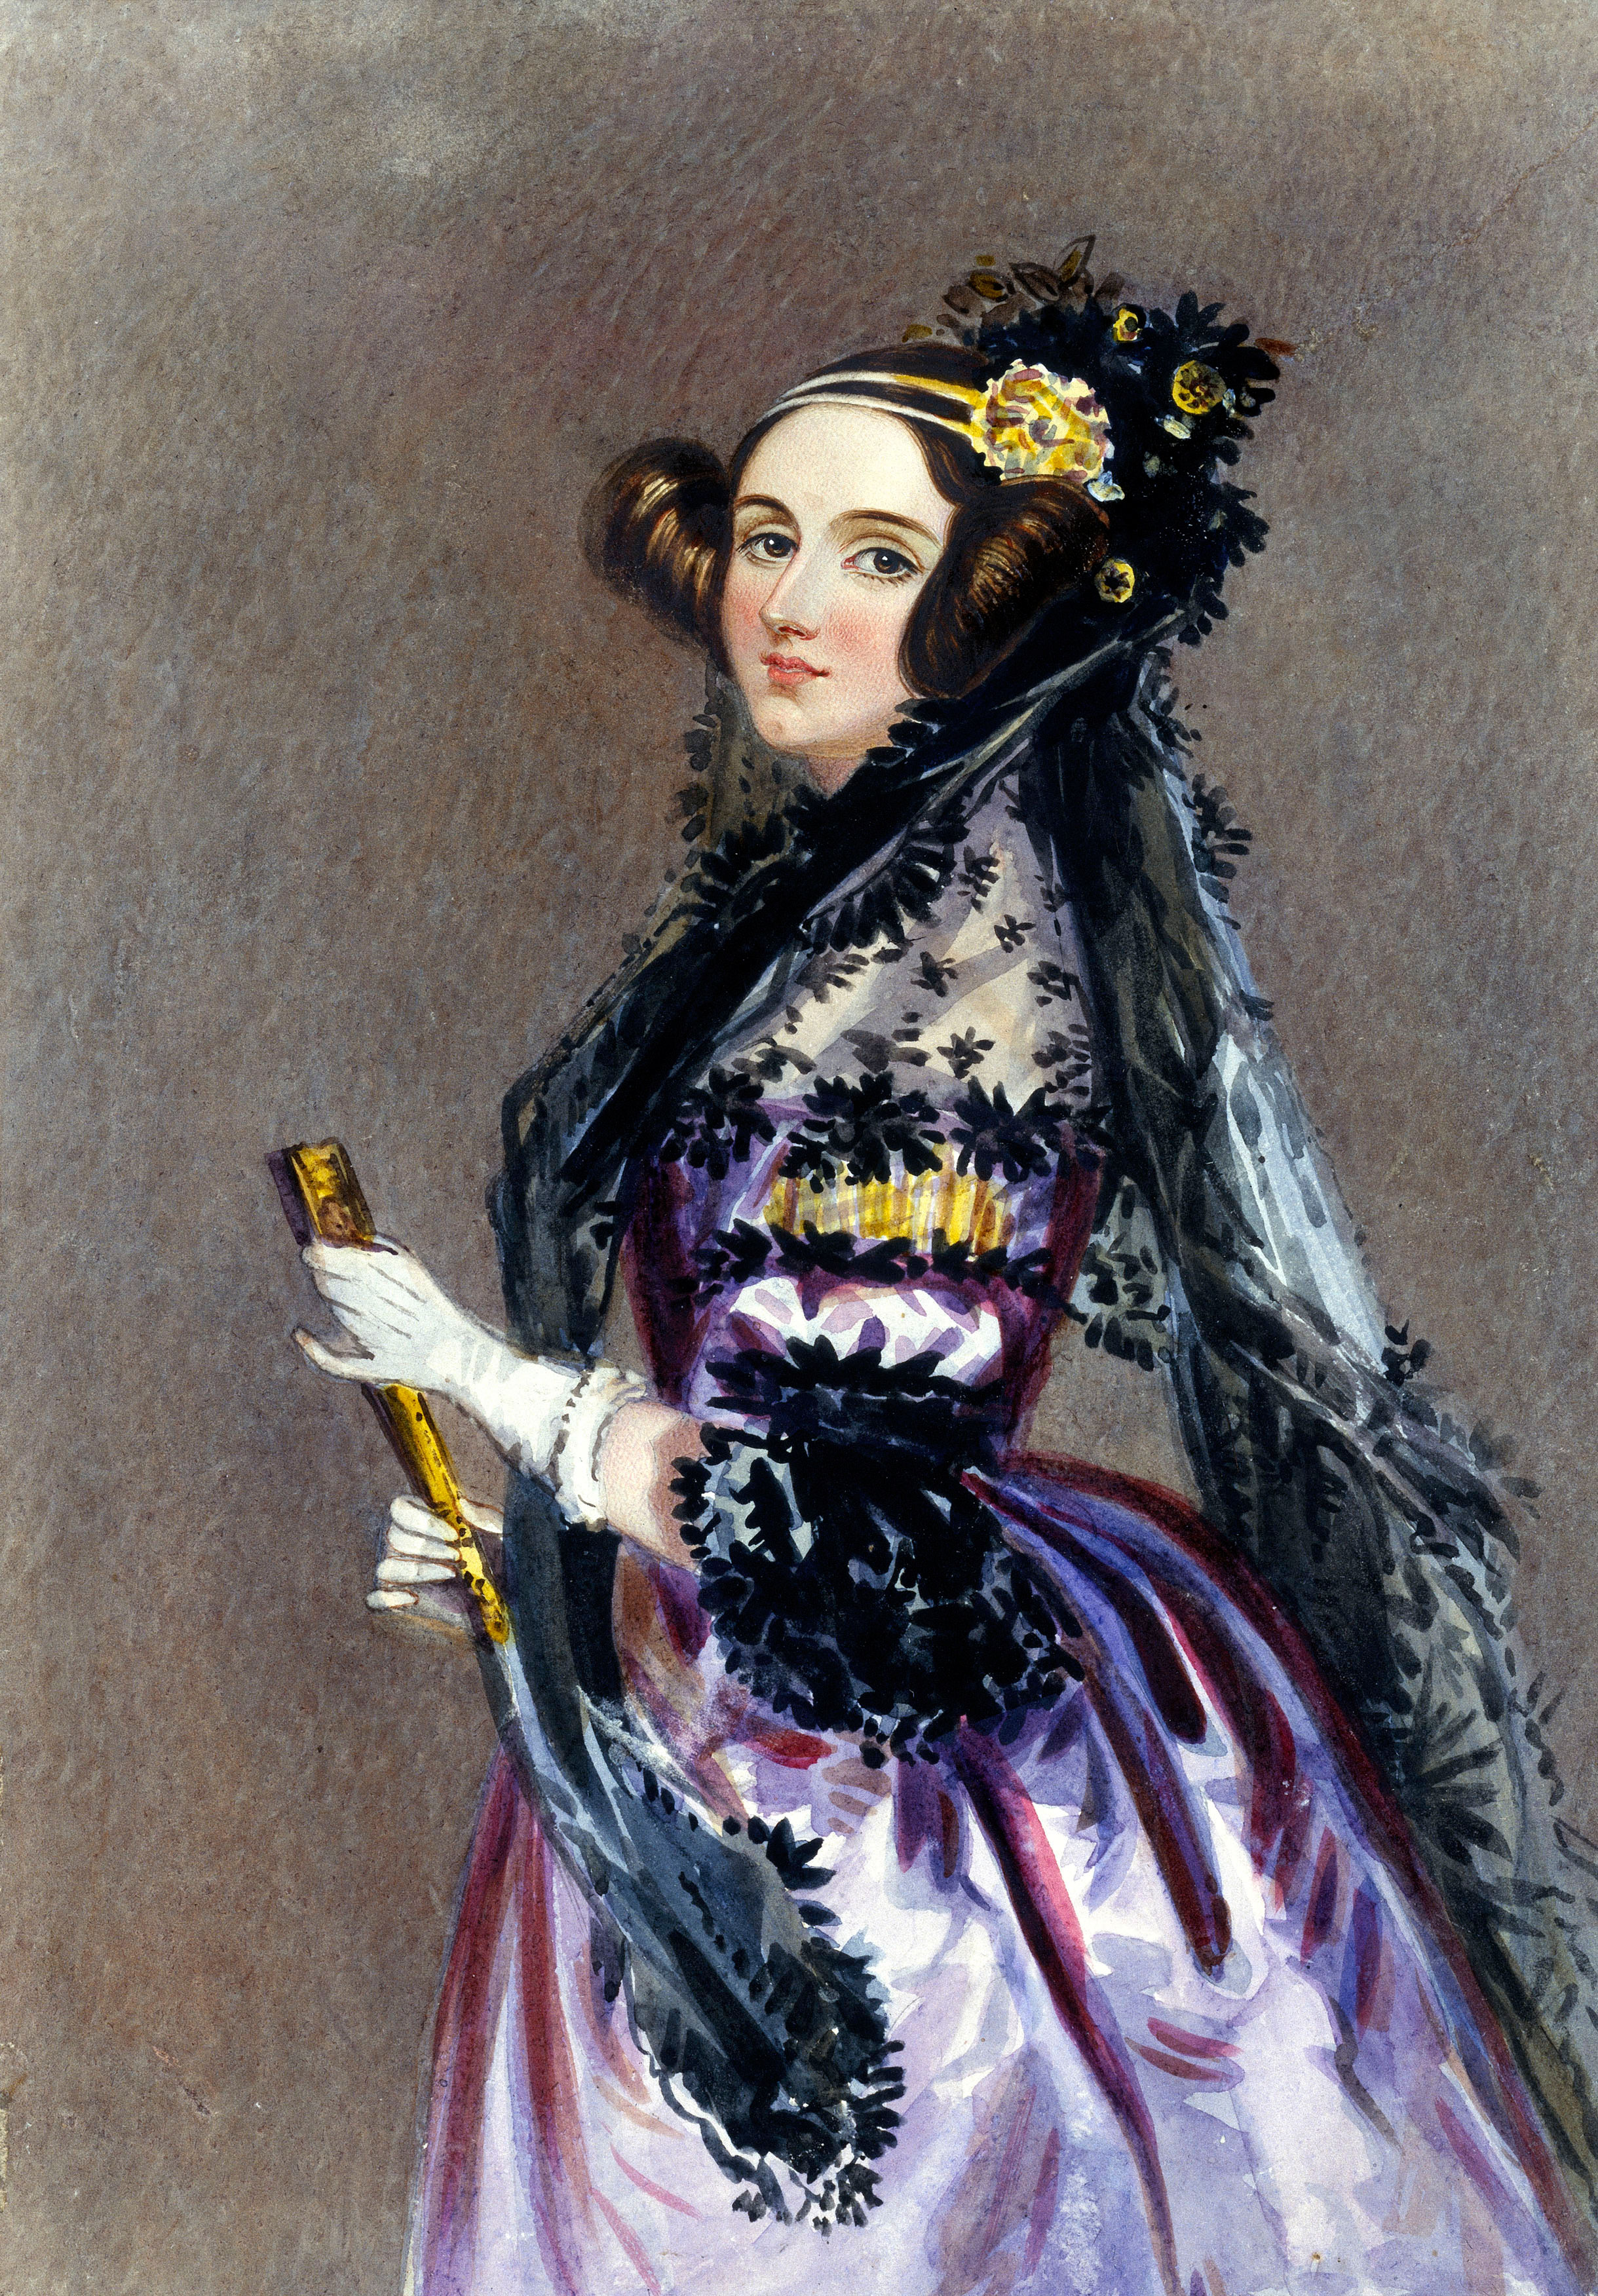
\includegraphics[width=0.4\linewidth]{AdaLovelace}
\label{fig:AdaLovelace}
\end{figure}

\end{frame}

\begin{frame}{The first programmable computer was the ENIAC,\\ used for scientific and military applications.}{}
\begin{figure}
\centering
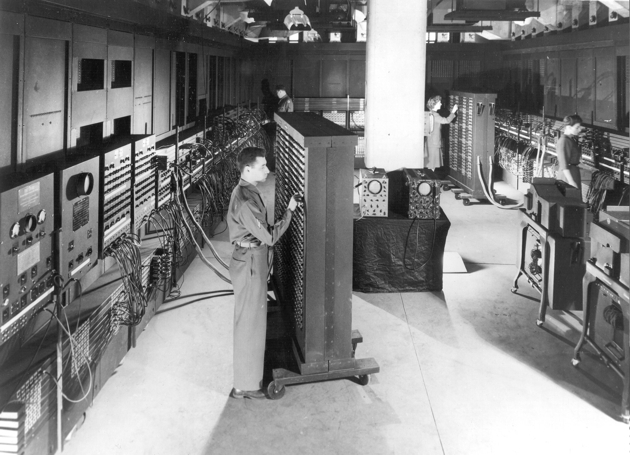
\includegraphics[width=0.7\linewidth]{ENIAC}
\label{fig:ENIAC}
\end{figure}
\end{frame}

\begin{frame}{Margaret Hamilton led the development of\\ the code for Apollo 11.}{}
\begin{figure}
\centering
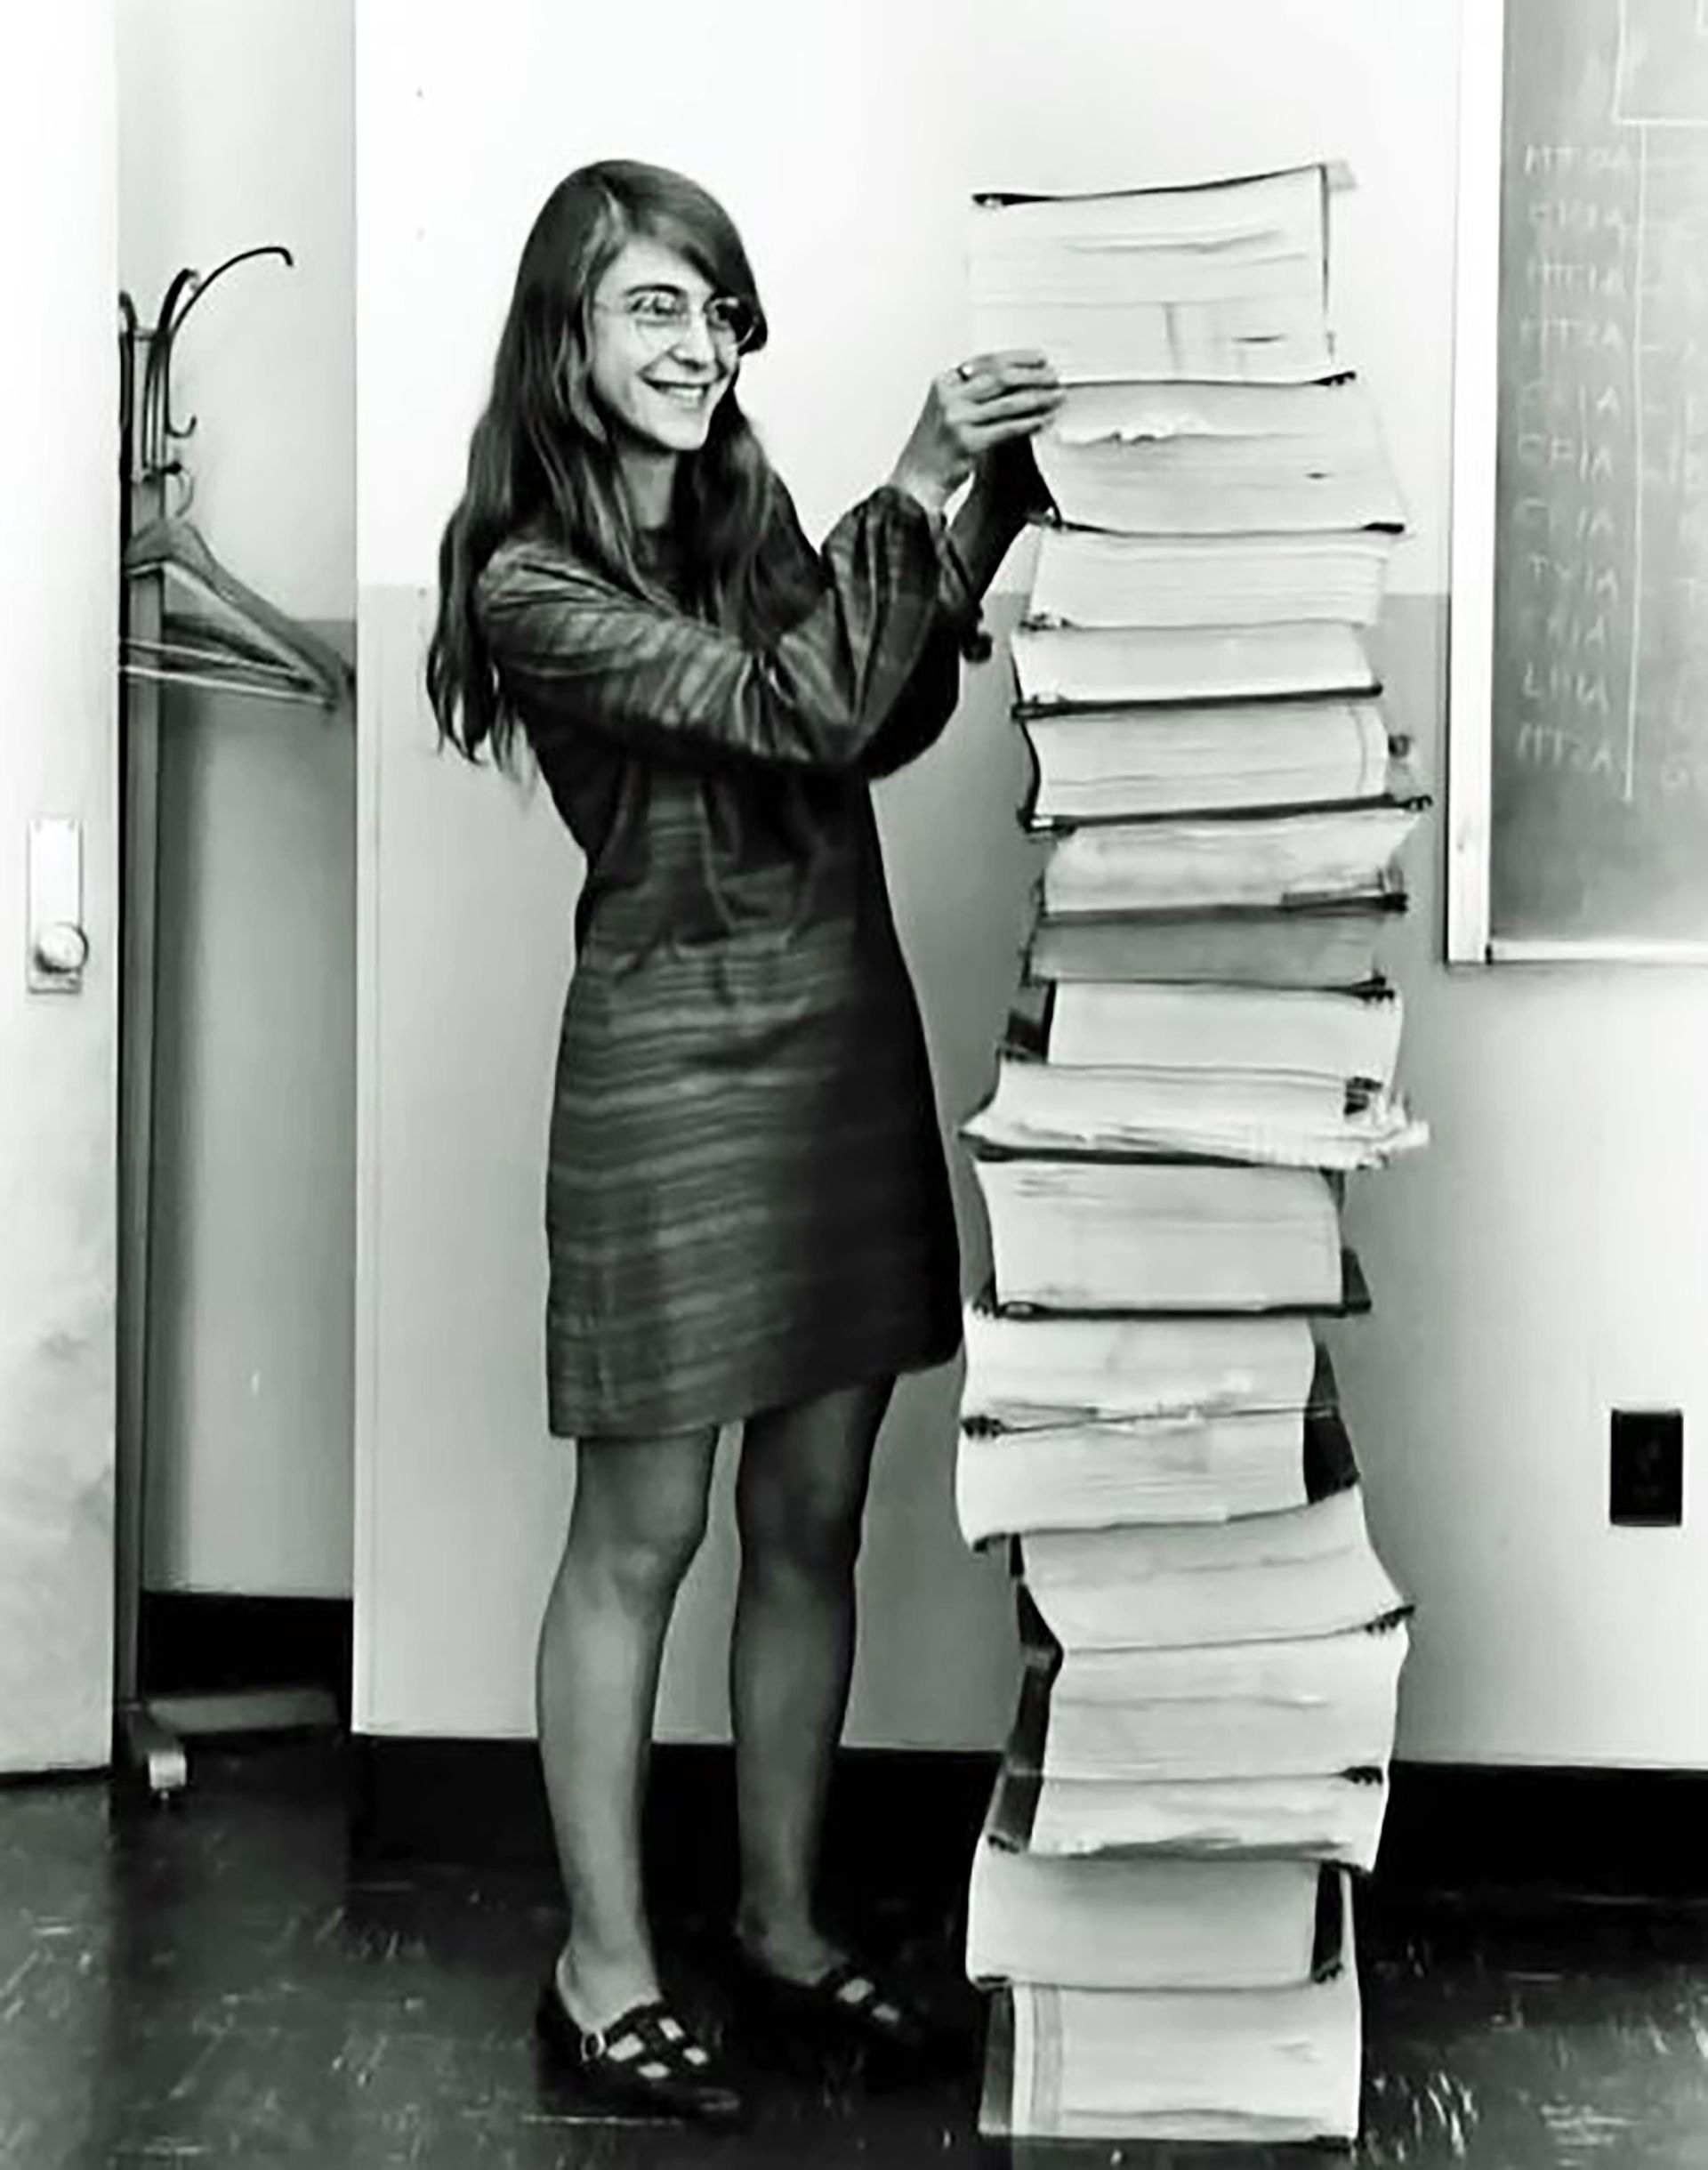
\includegraphics[height=0.7\textheight]{Apollo}
\label{fig:Apollo}
\caption*{\href{https://github.com/chrislgarry/Apollo-11}{This code is now available on GitHub.}}
\end{figure}
\end{frame}


\begin{frame}{Today we are using supercomputers\\ to simmulate black holes}{}
\begin{figure}[H]
\centering
\begin{subfigure}{.24\textwidth}
	\centering
	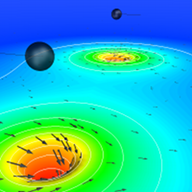
\includegraphics[width=\linewidth]{spec01}
\end{subfigure}
\begin{subfigure}{.24\textwidth}
	\centering
	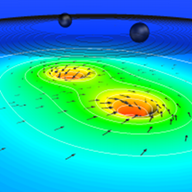
\includegraphics[width=\linewidth]{spec02}
\end{subfigure}
\begin{subfigure}{.24\textwidth}
	\centering
	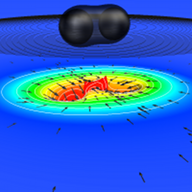
\includegraphics[width=\linewidth]{spec03}
\end{subfigure}
\begin{subfigure}{.24\textwidth}
	\centering
	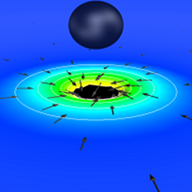
\includegraphics[width=\linewidth]{spec04}
\end{subfigure}
\label{fig:spec}
\caption*{\href{https://www.black-holes.org/SpEC.html}{\textbf{Spectral Einstein Code (SpEC)} simulation of inspiral and merger of two black holes.}}
\end{figure}
\end{frame}


\begin{frame}{Scientific Computing problems\\ may be classified into:}{}
\begin{itemize}[<+->]
\item \textbf{Root finding} Solve a system of equations
\item \textbf{Optimization} Maximize or minimize a cost function
\item \textbf{Modeling of data} Curve fitting, interpolation, extrapolation
\item \textbf{Numerical evaluation} Functions, series, derivatives, integrals
\item \textbf{Differential equations} Boundary Value Problems, Initial Value Problems
\end{itemize}
\end{frame}

\begin{frame}{Approaches of Scientific Computing}{}
\begin{itemize}[<+->]
	\item \textbf{Analytical} By hand, Computer Algebra Systems.
	\item \textbf{Numerical} Finite Differences, Spectral Methods.
	\item \textbf{Deterministic} Graphs, Dynamic Programming.
	\item \textbf{Heuristic} Montecarlo, Genetic Algorithms.
	\item \textbf{Machine Learning} Aritficial Neural Networks.
\end{itemize}
\end{frame}


\section{Tools and Environments}

\subsection{Methodology}

\begin{frame}{Solve the problem first,\\ then write code.}{}
Coding will always take an additional effort.

\pause
\bigskip
You may want to apply the \textbf{Feynman Algorithm} before writing the code:
\begin{enumerate}[<+(1)->]
\item Write down the problem.
\item Think real hard.
\item Write down the solution.
\end{enumerate}
\end{frame}

\subsection{Programming Languages}

\begin{frame}{High-level programming provides\\ the most straight-foward solutions}{}
A high-level approach relies on abstraction and a programming language rich in functions.

\bigskip
\begin{itemize}
\item \href{https://www.python.org/}{Python} (Fuctional)
\item \href{https://www.mathworks.com/products/matlab/}{MATLAB} (Numerical)
\item \href{https://www.comsol.com/multiphysics/finite-element-method}{COMSOL} (Finite Element Method)
\item \href{https://www.wolfram.com/mathematica/}{Mathematica} (Functional)
\end{itemize}
\end{frame}

\begin{frame}{Low-level programming provides\\ the most efficient solutions}{}
A low-level approach ussually requires more lines of code, but it is the way to achieve the most efficient solutions.

\bigskip
\begin{itemize}
\item \href{https://gcc.gnu.org/fortran/}{Fortran} (High perfomance computing, old school)
\item \href{http://www.cplusplus.com/doc/tutorial/}{C++} (Low-level memory management)
\item \href{http://www.oracle.com/technetwork/articles/javase/jdk-netbeans-jsp-142931.html}{Java} (Multi-platform applications)
\end{itemize}

\bigskip
Explicit data types and memory management.
\end{frame}


\subsection{Resources}
\begin{frame}{Commonly, your problem has already been solved\\ (or at least partially solved)}{}

The internet was invented for scientific collaboration. Google is your friend!
 
\bigskip
Here are some usefull sites
\begin{itemize}
\item \href{https://stackoverflow.com/}{Stack Overflow}
\item \href{http://stackexchange.com/}{Stack Exchage} (Super User, Mathematics, Physics)
\item \href{https://www.physicsforums.com/}{Physics Forums}
\item Online documentation
\end{itemize}
\end{frame}


\begin{frame}{Reference books}{}

\begin{itemize}
	\item \href{https://www.amazon.com/Java-Introduction-Problem-Solving-Programming/dp/0133766268/ref=sr_1_1?s=books&ie=UTF8&qid=1475804714&sr=1-1&keywords=Problem+solving+and+programming+Java}{\textbf{Problem solving and programming Java/C++} Savitch}
	\item \href{https://www.amazon.com/Numerical-Analysis-Richard-L-Burden/dp/1305253663/ref=sr_1_1?s=books&ie=UTF8&qid=1475804742&sr=1-1&keywords=numerical+analysis}{\textbf{Numerical Analysis} Burden and Faires}
	\item \href{https://www.amazon.com/Numerical-Recipes-3rd-Scientific-Computing/dp/0521880688/ref=sr_1_1?s=books&ie=UTF8&qid=1475804768&sr=1-1&keywords=Numerical+Recipes}{\textbf{Numerical Recipes} Press, Teukolsky et al}
	\item \href{https://www.amazon.com/Spectral-Methods-MATLAB-Software-Environments/dp/0898714656/ref=sr_1_1?s=books&ie=UTF8&qid=1475804790&sr=1-1&keywords=Spectral+Methods+in+MATLAB}{\textbf{Spectral Methods in MATLAB} Trefethen}
	\item \href{https://www.amazon.com/Computational-Science-Engineering-Gilbert-Strang/dp/0961408812/ref=sr_1_1?s=books&ie=UTF8&qid=1475804813&sr=1-1&keywords=Computational+Science+and+Engineering}{\textbf{Computational Science and Engineering} Strang}
	\item \href{https://www.amazon.com/Game-Physics-David-H-Eberly/dp/B003VIWRWW/ref=sr_1_2?s=books&ie=UTF8&qid=1475804827&sr=1-2&keywords=game+physics}{\textbf{Game Physics} Eberly}
\end{itemize}
	
\end{frame}

\begin{frame}{Popular Scientific Computing libraries}{}
User firendly
\begin{itemize}
	\item \textbf{\href{http://www.numpy.org/}{NumPy}, \href{https://www.scipy.org/}{SciPy}, \href{http://matplotlib.org/}{matplotlib}} (MATLAB inside Python)
	\item \href{http://arma.sourceforge.net/}{\textbf{Armadillo}} (MATLAB inside C++)
	\item \href{https://plot.ly/}{\textbf{Plotly}} (Online data visualization)
\end{itemize}

\pause
\bigskip
God tier
\begin{itemize}
	\item \href{https://www.gnu.org/software/gsl/}{\textbf{GSL}} GNU Scientific Library for C/C++
	\item \href{https://software.intel.com/en-us/intel-mkl}{\textbf{Intel MKL}} Math Kernel Library
	\item \href{http://www.netlib.org/blas/}{\textbf{BLAS}} and \href{http://www.netlib.org/lapack/}{\textbf{LAPACK}} Linear Algebra
	\item \href{http://www.fftw.org/}{\textbf{FFTW}} Fastest Fourier Transform in the West
	\item \textbf{\href{http://www.nvidia.com/object/cuda_home_new.html}{CUDA}, \href{https://www.khronos.org/opencl/}{OpenCL}} GPU programming
	\item \textbf{\href{https://www.opengl.org/}{OpenGL}, \href{https://www.khronos.org/vulkan/}{Vulkan}, \href{https://msdn.microsoft.com/en-us/library/windows/desktop/hh309466(v=vs.85).aspx}{Direct3D}} graphics
\end{itemize}
\end{frame}


\begin{frame}{Specialized Scientific Computing libraries}{}

\begin{itemize}
\item \href{http://www.chebfun.org/}{\textbf{Chebfun}} Numerical computing with functions
\item \href{http://persson.berkeley.edu/distmesh/}{\textbf{DistMesh}} Simple mesh generator in MATLAB
\item \href{https://www-user.tu-chemnitz.de/~potts/nfft/index.php}{\textbf{NFFT}} Non-equispaced Fast Fourier Transform
\item \href{http://www.caam.rice.edu/software/ARPACK/}{\textbf{ARPACK}} Large scale eigenvalue solver
\item \href{http://www.math.udel.edu/~driscoll/SC/}{\textbf{SCPACK}} Schwartz-Christoffel conformal mapping
\item \href{https://www.mathworks.com/matlabcentral/fileexchange/47844-multipareig}{\textbf{MultiParEig}} Multiparameter eigenvalue problem
\end{itemize}
\end{frame}




\section{Bondary Value Problems}

\begin{frame}{A Boundary Value Problem (BVP) \\ is a differential equation}{}

Find $u(x)$ that satifies a differential equation and boundary conditions. Example:

\bigskip
\begin{equation*}
\frac{d^2u}{dx^2}=1000cos(5\pi x)e^{-x^2}
\end{equation*}

\bigskip
With boundary conditions $u(-1)=2$ and $u(1)=-1$.
\end{frame}


\begin{frame}{Many natural-occuring BVPs are second order and linear}{}

Linear BVP (and some non-linear) may be discretized into matrix equations.
\begin{equation*}
A x = b
\end{equation*}

\bigskip
Numerical linear algebra has provided many succesfull methods for scientific computing problems.

\end{frame}


\end{document}


